\documentclass[11pt,a4paper]{article}

\usepackage[utf8]{inputenc}
\usepackage[T1]{fontenc}
\usepackage{lmodern}
\usepackage[margin=2.5cm]{geometry}
\usepackage{amsmath,amssymb}
\usepackage{tikz}
\usetikzlibrary{ positioning, arrows.meta, calc, fit, shapes.geometric }
\usepackage{hyperref}
\usepackage{booktabs}
\usepackage{listings}
\usepackage{xcolor}

\definecolor{codegreen}{rgb}{0,0.6,0}
\definecolor{codegray}{rgb}{0.5,0.5,0.5}
\definecolor{codepurple}{rgb}{0.58,0,0.82}
\definecolor{backcolour}{rgb}{0.95,0.95,0.92}
\definecolor{accent}{HTML}{27ae60}
\definecolor{accent2}{HTML}{2980b9}
\definecolor{accent3}{HTML}{e67e22}

\lstset{
  backgroundcolor=\color{backcolour},
  commentstyle=\color{codegreen},
  keywordstyle=\color{magenta},
  numberstyle=\tiny\color{codegray},
  stringstyle=\color{codepurple},
  basicstyle=\ttfamily\footnotesize,
  breaklines=true,
  captionpos=b,
  keepspaces=true,
  numbers=left,
  numbersep=5pt,
  showspaces=false,
  showstringspaces=false,
  tabsize=2
}

\title{Quick IPT --- Hidden-Point Measurement\\for the EVKA Position System}
\author{EVKA Position Project}
\date{\today}

\begin{document}
\maketitle

% ── What it is ────────────────────────────────────────────────────────────────
\section{What is Quick IPT?}

Quick IPT (Inverted Pen Technology) lets you \textbf{measure a point you cannot
touch directly} --- behind an obstacle, around a corner, inside a recess.  You
hold the pen \emph{tip} fixed on the hidden target and sweep the \emph{handle}
in a wide spiral.  The wire attaches to the pen body at a fixed offset $L$ from
the tip, so every point the sensor measures lies on a sphere of radius $L$
centred on the target.  Fitting that sphere recovers the target.

The method was pioneered by \textbf{Prodim International} in the
\textbf{Proliner V9} handheld 3D scanner (US Patent 9{,}267{,}794~B2).  The
Proliner V9 uses the same sensor topology as evka\_position: one draw-wire
encoder for length and two rotary encoders for angles.  This means the method
transfers directly --- \textbf{no firmware change is needed}; the entire feature
is a host-side Python tool that reads the live position stream and does the
math.

\begin{center}
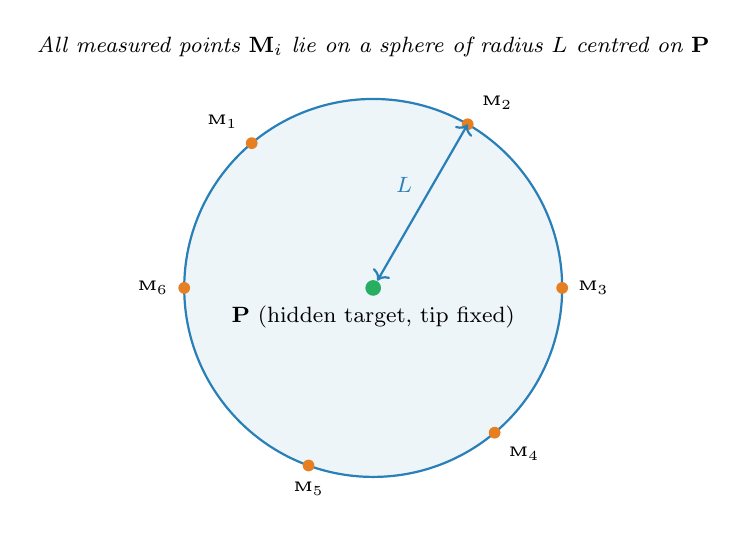
\begin{tikzpicture}[
  scale=1.0,
  every node/.style={font=\small},
  sphere/.style={circle, draw=accent2, fill=accent2!8, thick,
                 minimum width=4.8cm, minimum height=4.8cm},
  target/.style={circle, fill=accent, inner sep=2pt},
  mpt/.style={circle, fill=accent3, inner sep=1.5pt},
]
  % sphere
  \node[sphere] (s) at (0,0) {};
  % target (centre of sphere)
  \node[target, label={[font=\footnotesize]below:$\mathbf{P}$ (hidden target, tip fixed)}] (P) at (0,0) {};
  % measured points on the sphere surface
  \node[mpt, label={[font=\tiny]above left:$\mathbf{M}_1$}] at (130:2.4) {};
  \node[mpt, label={[font=\tiny]above right:$\mathbf{M}_2$}] at (60:2.4) {};
  \node[mpt, label={[font=\tiny]right:$\mathbf{M}_3$}] at (0:2.4) {};
  \node[mpt, label={[font=\tiny]below right:$\mathbf{M}_4$}] at (-50:2.4) {};
  \node[mpt, label={[font=\tiny]below:$\mathbf{M}_5$}] at (-110:2.4) {};
  \node[mpt, label={[font=\tiny]left:$\mathbf{M}_6$}] at (180:2.4) {};
  % radius arrow
  \draw[<->, thick, accent2] (P) -- (60:2.4)
    node[midway, above left, font=\footnotesize] {$L$};
  % label
  \node[above=0.4cm of s, font=\footnotesize\itshape]
    {All measured points $\mathbf{M}_i$ lie on a sphere of radius $L$ centred on $\mathbf{P}$};
\end{tikzpicture}
\end{center}

The core equation is simply:

\begin{equation}
  \|\mathbf{M}_i - \mathbf{P}\| = L \qquad \text{for every sample } i
\end{equation}

The solver fits the sphere to the measured point cloud and returns the centre
$\mathbf{P}$ --- the hidden target.  It also returns the fitted radius
$L_{\text{hat}}$, which \emph{self-calibrates} the pen offset: you never have to
measure $L$ precisely.

% ── Proliner context ──────────────────────────────────────────────────────────
\section{Proliner V9 and the same idea}

The \textbf{Prodim Proliner V9} is a portable 3D scanner for the stone, glass,
and metal fabrication industry.  The operator touches points with a pen
connected by a wire to a base unit.  The Proliner's \emph{Quick IPT} feature
extends this to hidden points: the pen tip stays fixed on the target while the
handle sweeps, and the device computes the sphere centre.

EVKA Position has the same sensor topology:

\begin{center}
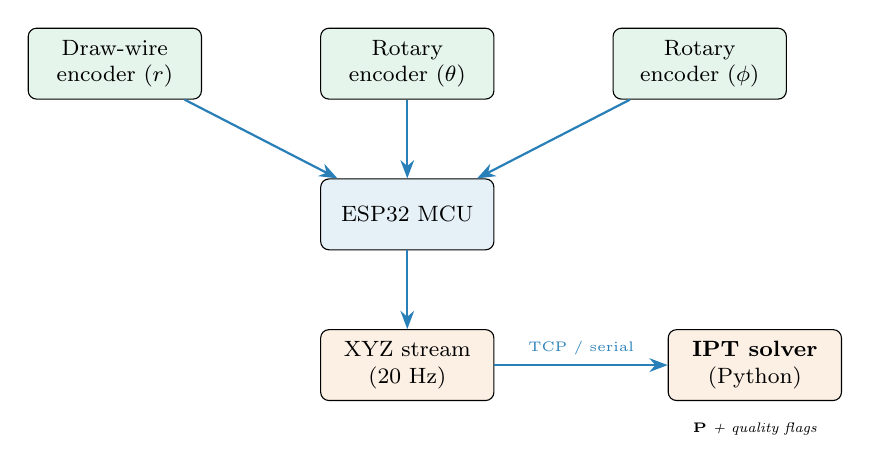
\begin{tikzpicture}[
  node distance=1.0cm and 1.5cm,
  box/.style={draw, rounded corners=3pt, minimum height=0.9cm,
              minimum width=2.2cm, align=center, font=\footnotesize},
  ar/.style={-Stealth, thick, accent2},
]
  \node[box, fill=accent!12] (wire) {Draw-wire\\encoder ($r$)};
  \node[box, fill=accent!12, right=of wire] (theta) {Rotary\\encoder ($\theta$)};
  \node[box, fill=accent!12, right=of theta] (phi) {Rotary\\encoder ($\phi$)};
  \node[box, fill=accent2!12, below=of theta] (mcu) {ESP32 MCU};
  \node[box, fill=accent3!12, below=of mcu] (out) {XYZ stream\\(20 Hz)};
  \node[box, fill=accent3!12, right=2.2cm of out] (ipt) {\textbf{IPT solver}\\(Python)};

  \draw[ar] (wire) -- (mcu);
  \draw[ar] (theta) -- (mcu);
  \draw[ar] (phi) -- (mcu);
  \draw[ar] (mcu) -- (out);
  \draw[ar] (out) -- (ipt)
    node[midway, above, font=\tiny] {TCP / serial};
  \node[below=0.15cm of ipt, font=\tiny\itshape] {$\mathbf{P}$ + quality flags};
\end{tikzpicture}
\end{center}

The Proliner V9 and EVKA Position both produce 3-DOF points (Cartesian XYZ),
not 6-DOF poses.  This is why multiple samples and a wide sweep are needed: the
sphere fit recovers the centre from the point cloud alone, without any
orientation information.

% ── How it works ──────────────────────────────────────────────────────────────
\section{How it works}

\subsection{The measurement}

\begin{enumerate}
\item \textbf{Connect} the Python tool to the EVKA device over TCP or serial.
\item Hold the pen \textbf{tip} firmly on the hidden target.
\item Click \textbf{ARM} and sweep the handle in a \textbf{wide spiral}.
\item Click \textbf{STOP}, then \textbf{SOLVE}.
\end{enumerate}

\begin{center}
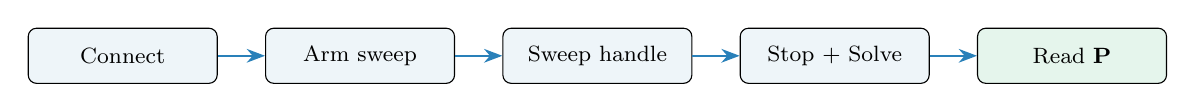
\begin{tikzpicture}[
  node distance=0.6cm,
  stage/.style={draw, rounded corners=3pt, fill=accent2!8,
                minimum width=2.4cm, minimum height=0.7cm, font=\footnotesize},
  ar/.style={-Stealth, thick, accent2},
]
  \node[stage] (s1) {Connect};
  \node[stage, right=of s1] (s2) {Arm sweep};
  \node[stage, right=of s2] (s3) {Sweep handle};
  \node[stage, right=of s3] (s4) {Stop + Solve};
  \node[stage, right=of s4, fill=accent!12] (s5) {Read $\mathbf{P}$};
  \draw[ar] (s1) -- (s2);
  \draw[ar] (s2) -- (s3);
  \draw[ar] (s3) -- (s4);
  \draw[ar] (s4) -- (s5);
\end{tikzpicture}
\end{center}

\subsection{Two solver modes}

\begin{itemize}
\item \textbf{Self-calibrating} (leave L blank): fits both centre and radius.
  $L_{\text{hat}}$ is the fitted pen length --- should match your physical pen
  within a few mm.
\item \textbf{Known L} (enter pen length): uses a better-conditioned trilateration
  method.  $L_{\text{used}}$ is the value you entered; $L_{\text{fit}}$ is the
  independent sphere-fit radius --- if they differ by more than a few mm, the
  entered length is wrong or the tip slipped.
\end{itemize}

\subsection{Quality flags}

\begin{center}
\begin{tabular}{@{}lll@{}}
\toprule
Flag & Metric & Bands \\
\midrule
\textbf{slip\_warning} & RMS residual &
  ok $<$ 2\,mm,\;\; warn 2--5\,mm,\;\; reject $>$ 5\,mm \\[3pt]
\textbf{geom\_warning} & Geometric condition &
  ok $<$ 150,\;\; warn 150--1500,\;\; block $>$ 1500 \\
\bottomrule
\end{tabular}
\end{center}

\textbf{RMS residual} tells you if the tip slipped.  \textbf{Geometry cond}
tells you if the sweep was too small.  Both are heuristic thresholds tuned in
simulation --- re-tune on real hardware.

\begin{center}
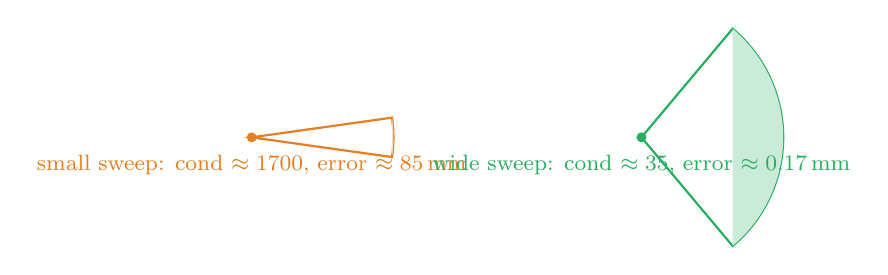
\begin{tikzpicture}[scale=0.9, every node/.style={font=\footnotesize}]
  % small sweep
  \draw[accent3, thick] (0,0) -- (8:2) arc (8:-8:2) -- cycle;
  \fill[accent3!30] (8:2) arc (8:-8:2) -- cycle;
  \node[below=0.1cm of {(0,0)}, accent3] {small sweep: cond $\approx 1700$, error $\approx 85$\,mm};
  \fill[accent3] (0,0) circle (2pt);

  % big sweep
  \begin{scope}[xshift=5.5cm]
    \draw[accent, thick] (0,0) -- (50:2) arc (50:-50:2) -- cycle;
    \fill[accent!25] (50:2) arc (50:-50:2) -- cycle;
    \node[below=0.1cm of {(0,0)}, accent] {wide sweep: cond $\approx 35$, error $\approx 0.17$\,mm};
    \fill[accent] (0,0) circle (2pt);
  \end{scope}
\end{tikzpicture}
\end{center}

A small patch of a large sphere is nearly flat --- it cannot pin the centre.
This is geometric dilution of precision, exactly like poor satellite geometry in
GNSS.  \textbf{Sweep wider.}

% ── Implementation ────────────────────────────────────────────────────────────
\section{Implementation}

\begin{center}
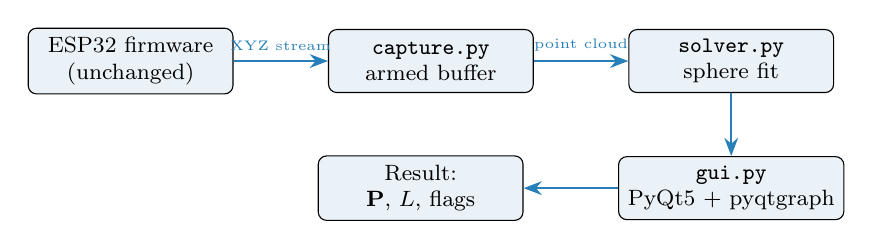
\begin{tikzpicture}[
  node distance=0.8cm and 1.2cm,
  mod/.style={draw, rounded corners=3pt, fill=accent2!10,
              minimum width=2.6cm, minimum height=0.8cm,
              align=center, font=\footnotesize},
  ar/.style={-Stealth, thick, accent2},
]
  \node[mod] (firm) {ESP32 firmware\\(unchanged)};
  \node[mod, right=of firm] (cap) {\texttt{capture.py}\\armed buffer};
  \node[mod, right=of cap] (sol) {\texttt{solver.py}\\sphere fit};
  \node[mod, below=of sol] (gui) {\texttt{gui.py}\\PyQt5 + pyqtgraph};
  \node[mod, left=of gui] (out) {Result:\\$\mathbf{P}$, $L$, flags};

  \draw[ar] (firm) -- node[above, font=\tiny] {XYZ stream} (cap);
  \draw[ar] (cap) -- node[above, font=\tiny] {point cloud} (sol);
  \draw[ar] (sol) -- (gui);
  \draw[ar] (gui) -- (out);
\end{tikzpicture}
\end{center}

The code lives in \texttt{tools/ipt/} --- a small Python package:

\begin{lstlisting}[language=bash]
tools/ipt/
  __main__.py   # CLI: python -m tools.ipt --tcp 192.168.1.50:8080
  solver.py     # Sphere fit + trilateration + Gauss-Newton (pure numpy)
  capture.py    # Armed buffer: dedup, validity, finite-value guard
  gui.py        # PyQt5 window: 3D cloud, fitted sphere, controls
  tests/        # Offline pytest suite (no hardware needed)
\end{lstlisting}

\textbf{No firmware upload.}  The tool connects to the existing EVKA device and
reads the live 20\,Hz position stream.  The ESP32 code is unchanged.

\subsection*{Transport asymmetry}

The firmware sends different line formats over serial vs.\ TCP:

\begin{itemize}
\item \textbf{Serial:} one \texttt{DATA,...} line per cycle (XYZ + validity).
\item \textbf{TCP:} separate \texttt{X,Y,Z} and \texttt{SENSOR,...} lines.
  The capture buffer pairs them to recover validity.
\end{itemize}

At 20\,Hz the firmware emits many near-identical frames when the handle is still.
The buffer deduplicates points closer than 1\,mm to the last accepted sample.

% ── Usage ─────────────────────────────────────────────────────────────────────
\section{How to use it}

\begin{lstlisting}[language=bash]
# WiFi (connect to CMDCNC_EVKA AP at 192.168.1.50)
python -m tools.ipt --tcp 192.168.1.50:8080

# Serial
python -m tools.ipt --serial /dev/ttyUSB0 --baud 115200

# No flag -- opens disconnected, pick transport in the panel
python -m tools.ipt
\end{lstlisting}

Then: connect, hold tip on target, ARM, sweep wide, STOP, SOLVE.

The recovered point $\mathbf{P}$ is in the \textbf{sensor origin frame} (the boot
zero-point), in mm --- the same frame as the live X/Y/Z readout, not a world
frame.

% ── Limitations ───────────────────────────────────────────────────────────────
\section{Limitations}

\begin{itemize}
\item \textbf{3-DOF only.} No orientation sensor; IPT recovers the hidden
  \emph{point}, not a 6-DOF pose.
\item \textbf{Tip slip.} RMS residual flags it but cannot fix it. Re-measure.
\item \textbf{Sweep geometry.} Small sweeps give poor conditioning. The
  \texttt{geom\_warning} flag is your cue to sweep wider.
\item \textbf{Coordinate frame.} Results are relative to the sensor's boot
  zero-point. If the sensor is moved or re-zeroed, the recovered target is no
  longer valid.
\end{itemize}

% ── IP note ───────────────────────────────────────────────────────────────────
\section*{Intellectual property note}

The Quick IPT method is patented by Prodim International
(US~9{,}267{,}794~B2, EP~2{,}792{,}994~B1).  This implementation is a technical
reverse-engineering exercise for research and educational purposes.  The
mathematical methods (sphere fitting, pivot calibration) are well-established
in the literature.  Commercial deployment may require licensing from Prodim.

% ── References ─────────────────────────────────────────────────────────────────
\begin{thebibliography}{9}
\bibitem{yaniv2015}
  Z.~Yaniv,
  ``Which Pivot Calibration?'',
  \emph{SPIE Medical Imaging}, vol.~9415, 2015.
\bibitem{coope1993}
  I.~D.~Coope,
  ``Circle fitting by linear and nonlinear least squares'',
  \emph{J.~Opt.\ Theory Appl.}, vol.~76, no.~2, pp.~381--388, 1993.
\bibitem{prodim2016}
  E.~Teune and J.~Janssen,
  ``Method and device for determining a position of a measurement tip'',
  US Patent 9{,}267{,}794~B2, 2016.
\end{thebibliography}

\end{document}
